% vim: set tw=0:
\documentclass{beamer}
\usepackage{graphicx}
\usepackage{hyperref}
\hypersetup{pdfborder={0 0 0 0}}

% Reasonable themes:
% Antibes Bergen Berkeley Berlin Frankfurt Goettingen Ilmenau Luebeck Malmoe
% Montpellier PaloAlto Rochester Singapore Szeged Warsaw bars boxes
% compatibility default lined plain shadow sidebar split tree
% And these ones include the author's name on every slide:
% Berkeley

% Declare themes.
\mode<presentation>
\usetheme{UWHEP}

% Personal macros.
\newcommand{\email}[1]{{\texttt #1}}
\newcommand{\newframe}[1]{\section{#1}
    \frametitle{\sc{#1}}}
\newcommand{\subframe}[1]{\subsection{#1}
    \frametitle{\sc{#1}}}
\newcommand{\supers}[1]{\ensuremath{^\textrm{#1}}}
\newcommand{\subs}[1]{\ensuremath{_\textrm{#1}}}
\newcommand{\ca}{\ensuremath{\sim}}
\renewcommand{\email}[1]{\href{mailto:#1}{\nolinkurl{#1}}}

% Author information.
\title{T2 Status}
\author[Maier, Mohapatra]{
    Will Maier \and Ajit Mohapatra\\ 
    {\tt wcmaier@hep.wisc.edu}\\
    {\tt ajit@hep.wisc.edu}}
\institute[Wisconsin]{University of Wisconsin - High Energy Physics}
\date{2009.08.18}
\logo{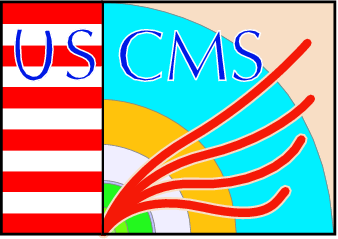
\includegraphics[height=0.6cm]{../../../Graphics/USCMS_logo.png}\hspace{.1cm}
\includegraphics[height=0.75cm]{../../../Graphics/UW_logo.png}}

\begin{document}

\begin{frame}
    \titlepage
\end{frame}

%\section{Overview}
%\begin{frame}
%    \tableofcontents
%\end{frame}

\section{Facilities}
\subsection{Software and Storage}
\begin{frame}
\frametitle{}

\begin{itemize}
	\item Current resources: 3.5 kSI2K, 250 TB writable space
	\begin{itemize}
		\item Plan to deploy more storage in September/October
	\end{itemize}
	\item SL5 tested, pushing to racks this week and next
	\item Enabled extra priority for US users
	\item Delayed OSG 1.2 upgrade due to reported bugs, SL5 conversion plans
	\item Deployed 40 8-core Harpertowns (opportunistic with high priority)
	\item Fixed faulty termination in Cisco switch stack (full backplane bandwidth)
	\item PNFS upgrade successful; 20\% performance gain
	\item AFS server upgrade complete
	\item Planning network upgrade (before data taking?): 4 x 10 Gbps fiber uplinks to campus
\end{itemize}

\end{frame}

\subsection{Production and Monitoring}
\begin{frame}
\frametitle{}
\begin{itemize}
	\item JobRobot: OK
	\item SAM: OK
	\item RSV: OK
	\item PhEDEx:
	\begin{itemize}
		\item Uplinks: US T2s, SPRACE; downlinks: US T2s (except MIT) SPRACE
		\item Usual MC transfers for local users
		\item dCache is getting full -- need to clean up
	\end{itemize}
	\item MC Production:
	\begin{itemize}
		\item Summer09 production contiues: 200M Fullsim in 20 days, pretty good resource utilization both in OSG and LCG
		\item Another 60M at 10 TeV to go in the first round (hopefully within this month)
		\item Will likely have to re-produce all the samples with 7TeV configs
	\end{itemize}
	\item DataOps
	\begin{itemize}
		\item Inefficient: samples produced in the US sometimes end up at LCG T1s (transferred via FNAL)
		\item Instead, provision US T2 - LCG T1 uplinks
		\item Will ask DDT for help
	\end{itemize}
\end{itemize}
\end{frame}

\end{document}
